\documentclass{article}
\usepackage[margin=0.5in]{geometry}
\usepackage{hyperref}
\usepackage{amsmath}
\usepackage{amsfonts}
\usepackage{tikz}
\usepackage{graphicx}
\usetikzlibrary{automata,positioning}
\title{Dynamic Branch Prediction Using Perceptrons}
\author{Andrew Bruce \\ \href{mailto:acbruce@ucsc.edu}{acbruce@ucsc.edu}
  \and Gowrav BG \\ \href{mailto:gbukkapa@ucsc.edu}{gbukkapa@ucsc.edu} }

\begin{document}
\maketitle
\pagenumbering{gobble}
\section*{Goal}
\indent We aim to implement a dynamic branch predictor that uses a perceptron to adapt its weights at runtime using the perceptron training algorithm based off the 2 bit prediction history register \cite{article}.
\section*{Implementation}
\indent We would need to create a custom branch predictor using the \verb=Bp_struct=. The history register is already handled, and we would need to use it as a ``two-level adaptive predictor'', and keep track of the counter for each of the possible 4 histories. The perceptron would then take the counters in each history of the table as counters. In theory each branch would need its own perceptron, but in practice we would just index a table of perceptrons based off a hash of the branch address. For the hash function we would plan to just take the branch address and modulus it by the size of the table. Each perceptron would need four weights, one for each of the histories. The global history is already implemented in Scarab inside the \verb=Bp_Data_struct= struct as other branch prediction algorithms use it, so we would just need to implement the required functions for the custom branch predictor.\\
\indent The global history table should look like:
\begin{center}
  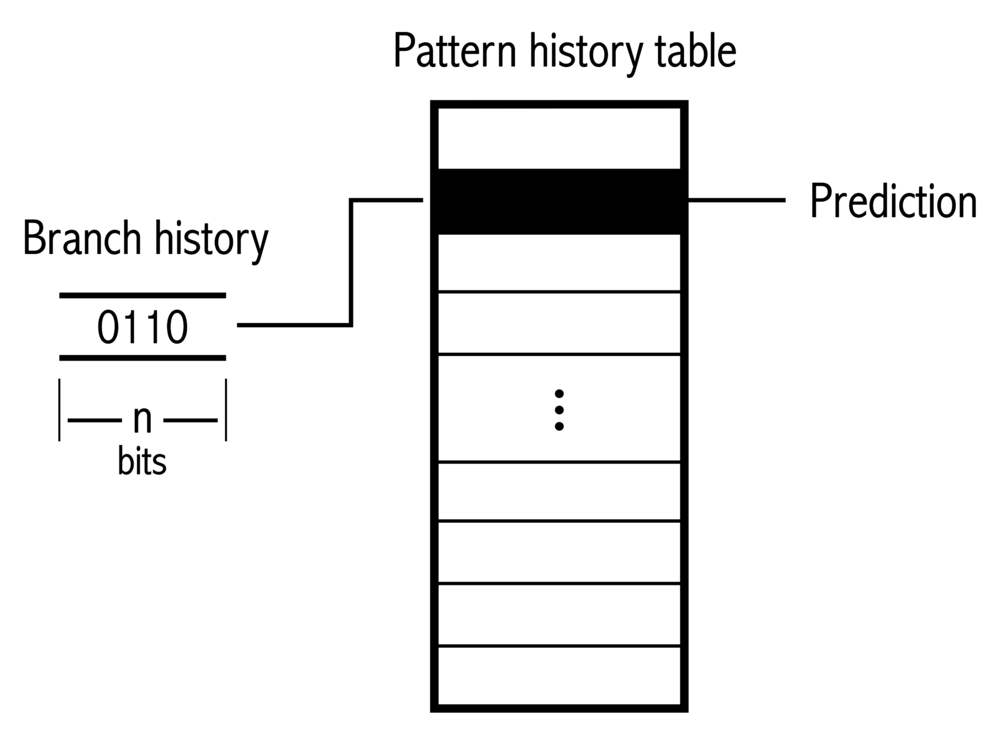
\includegraphics[width=0.3\textwidth]{table.png}
\end{center}
\indent Then each entry in the perceptron hash table will contain a perceptron that looks like:
\begin{center}
  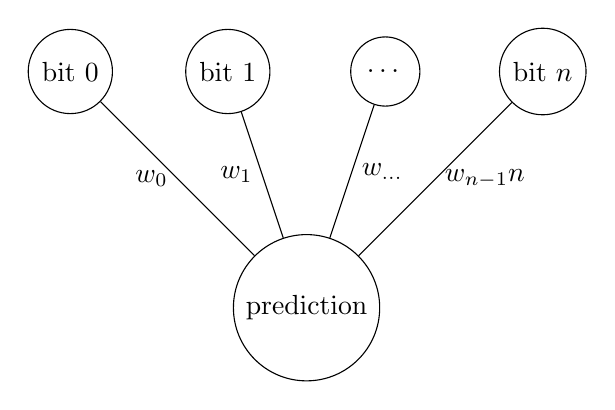
\begin{tikzpicture}
    \node[state] (q1) at (0,3) {bit 0};
    \node[state] (q2) at (2,3) {bit 1};
    \node[state] (q3) at (4,3) {\dots};
    \node[state] (q4) at (6,3) {bit $n$};
    \node[state] (q5) at (3, 0) {prediction};
    \draw (q1) edge [left=10pt] node {$w_0$} (q5)
    (q2) edge [left=10pt] node {$w_1$} (q5)
    (q3) edge [right=10pt] node {$w_{\dots}$} (q5)
    (q4) edge [right=10pt] node {$w_{n-1}n$} (q5);
  \end{tikzpicture}
\end{center}
\indent We will only be using $n = 2$ bits in the history buffer, so we will only have 2 weights. The inputs will be either $-1$ or $1$ based on the history bit. The calculation will look like
\begin{center}
  $y = b + \sum_{i = 0}^{n-1}w_{i} \times \text{bit } i$
\end{center}
where $b, y, w_i \in \mathbb{R}$ and $\text{bit } i \in \{-1, 1 \}$. The final prediction will be the sign bit of $y$. The perceptron training algorith is the the same as classic machine learning algorithms:
\begin{verbatim}
if (sign(y) != real) || (|y| <= threshold){
  for(int i = 0; i++; i < n){
    w_i = w_i + t*x_i;
  }
  b = t*x_i;
}
\end{verbatim}
\indent We would need to implement the prediction and training algorithm in the \verb=Bp_struct=
\begin{verbatim}
typedef struct Bp_struct {
  Bp_Id       id;
  const char* name;
  void (*init_func)(void);       /* called to initialize the predictor */
  void (*timestamp_func)(Op*);   /* called to timestamp a branch for prediction,
                                    update, and recovery */
  uns8 (*pred_func)(Op*);        /* called to predict a branch instruction */
  void (*spec_update_func)(Op*); /* called to update the speculative state of
                                    the predictor in the front-end */
  void (*update_func)(Op*); /* called to update the bp when a branch is resolved
                               (at the end of execute or retire) */
  void (*retire_func)(Op*); /* called to retire a branch and update the state of
                               the bp that has to be updated after retirement*/
  void (*recover_func)(Recovery_Info*); /* called to recover the bp when a
                                           misprediction is realized */
  uns8 (*full_func)(uns);
} Bp;
\end{verbatim}
by making the \verb=pred_func= run inference, and the \verb=update_func= with the perceptron training algorithm.
\bibliographystyle{abbrv}
\bibliography{refs}
\end{document}
